\chapter{Stavba siete} \label{stavba}

Všetky siete boli napísané v programovacom jazyku \textit{Python} s použitím knižníc \textit{numpy} a \textit{tensorflow}.
Na vylepšovanie siete sme, ako je napísané v kapitole \ref{docu}, použili údaje, ktoré sa napokon budú pri vyhodnocovaní nachádzať medzi trénovacími dátami. 

Konkrétne, pre futbal dáta predstavovali 7 celých sezón a prvú polovicu ďalšej sezóny (ako popísané v \ref{foot}), vyhodnocovacie dáta predstavujú druhú polovicu tejto sezóny. 
Takže sme trénovacie dáta rozdelili na tri časti, 6 celých sezón a polovicu ďalšej (trénovacie dáta), druhú polovicu siedmej sezóny (testovacie dáta) a zvyšnú prvú polovicu ôsmej sezóny (nepoužité dáta).

V prípade tenisu prišli dáta už priamo z transformačnej časti v troch súboroch, trénovacie, testovacie a vyhodnocovacie dáta.

Každá sieť mala svoje nedostatky v celkovej úspešnosti, ale doposiaľ neexistuje efektívne nastavenie neurónových sietí pre každú situáciu \citep{gitgud}, takže každá sieť sa musela vylepšovať osobitne a manuálne vzhľadom na rozdiely v prístupoch.

\section{Selekcia príznakov}
Kliatba dimenzionality nám hovorí, že čím viac vstupných príznakov zadáme neurónovej sieti, tým sú dáta redšie a teda je ich potreba získať viac, aby sa sieť správne učila. Viac dát získať nevieme, takže sa pokúsime znížiť počet dimenzií a pozrieť sa na to, ako sa to prejaví na trénovacích dátach.
Na začiatok spravíme korelačný test všetkých príznakov testovacích a trénovacích dát (obrázky \ref{corr} a \ref{corr_atp}).
Teória hovorí, že by nám mohla napovedať, aké hodnoty sú dôležité.
Obrázok \ref{corr} týkajúci sa futbalu hovorí, že najvyššiu koreláciu s výsledkom zápasu majú príznaky 41 a 42 určujúce dlhodobú silu tímu. Skóre dosahuje tiež celkom vysokú koreláciu (okolo 0,2) s finálnym výsledkom.
\noindent
\begin{figure}  [h!]
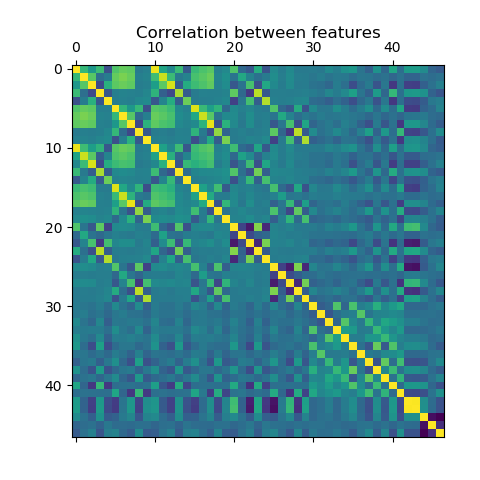
\includegraphics[scale=0.9]{../img/correng.png}
\caption{Korelačná tabuľka všetkých príznakov pre anglickú Premier League, žltá predstavuje kladnú koreláciu, modrá zápornú. Nás hlavne zaujímajú posledné 3 riadky určujúce koreláciu príznaku s výsledkom zápasu (príznaky sú v poradí ako v Prílohe \ref{in:foot}).}
\label{corr} 
\end{figure}

V prípade tenisu obrázok \ref{corr_atp} naznačuje najvyššiu koreláciu medzi výsledkom a oboma druhmi skóre, veľkú rolu zohráva postavenie v rebríčku ATP a vzájomné zápasy (konkrétne priemerný rozdiel v počte vyhraných gemov za set).

\begin{figure} [h!]
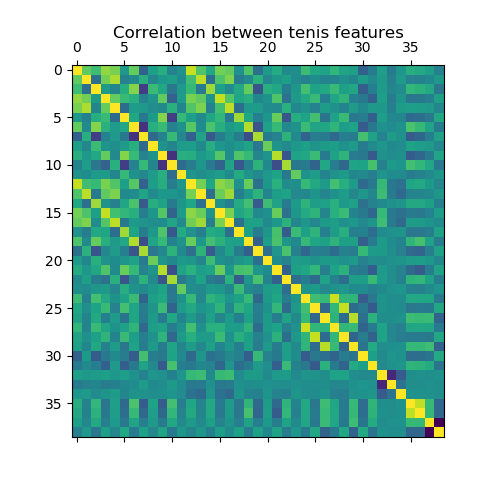
\includegraphics[scale=0.9]{../img/corratp.png}
\caption{Korelačná tabuľka všetkých príznakov pre tenisové zápasy, žltá predstavuje kladnú koreláciu, modrá zápornú. Nás hlavne zaujímajú posledné 2 riadky určujúce koreláciu príznaku s výsledkom zápasu (príznaky sú v poradí ako v Prílohe \ref{in:foot}).}
\label{corr_atp}
\end{figure}

Tieto tabuľky boli pre nás viac-menej informačné.
Korelovanosť jedného príznaku s výsledkom nám nemusí hovoriť nič.
Stačí sa pozrieť na funkciu XOR (tabuľka \ref{xor}). Ak by sme na hodnoty v tejto tabuľke aplikovali koreláciu, tak by sme sa dozvedeli, že x, y a ani hodnota x $XOR$ y nemajú po dvoch žiadnu koreláciu (ak vieme, akú hodnotu má x, nijak to pre nás nemení pravdepodobnosť, že x XOR y bude napríklad 0). Až kombinácia hodnôt x a y priamo určuje hodnoty funkcie XOR.
Selekcia príznakov, s ktorými dosahovala sieť najlepšie trénovacie výsledky a ktoré budú použité na získanie výsledkov v kapitole \ref{res}, bol uskutočnený spôsobom pokus-omyl, keďže nič lepšie nevieme, ako už bolo spomínané na začiatku kapitoly.

\section{Proces tréningu} \label{train}
Proces tréningu siete začínal základným nastavením siete, ktoré je presnejšie popísané v nasledujúcich kapitolách, pretože pre každú sieť bolo unikátne.
Po trénovaní siete v základnom nastavení nasledovalo spustenie siete na testovacích dátach.
Nasledoval pokus nastaviť parametre (tie budú tiež popísané v nasledujúcich sekciách, líšili sa pre jednotlivé druhy neurónových sietí) jednotlivých sietí pre každý šport a ligu tak, aby dosahovali čo najvyššie sledované hodnoty.
Tieto hodnoty predstavovali referenčnú hodnotu, ktorú sme chceli selektovaním jednotlivých parametrov vylepšiť.
Následne sme vybrali jednu z podmnožín príznakov (napríklad odstránili údaje o forme) a opakovali proces vylaďovania parametrov.
Na konci pre každú sieť ostala jedna podmnožina príznakov a nastavenie parametrov siete, ktoré v kombinácii s ňou vydávalo najlepšie výsledky v sledovaných oblastiach.

Sledované oblasti zo začiatku predstavovali trénovaciu a testovaciu úspešnosť, úspešnosť v zápasoch bez favorita a eventuálny zisk, ktorý by sme dosiahli, ak by sme v týchto zápasoch uzatvárali stávky podľa nápovedy danej siete. 
Všetky modely ale ukazovali veľmi podobnú úspešnosť v tipovaní víťazov zápasov bez favorita (napríklad pri vytváraní siete pre tipovanie anglickej futbalovej Premier League vydávali všetky siete trénovaciu úspešnosť 36--39\%).
Eventuálny zisk osciloval bez ohľadu na túto úspešnosť.
Neobjavil som žiadnu koreláciu medzi nastavenými parametrami, selektovanými príznakmi a týmto ziskom, takže predpokladám, že na hodnote tohto údaja pri trénovaní až tak nezáleží, pretože vo vyhodnocovacom procese môže dosiahnuť úplne iné výsledky.
Nakoniec teda som sledované oblasti zúžil na trénovaciu a testovaciu úspešnosť, kde som sa pokúšal maximalizovať testovaciu úspešnosť a trénovacia slúžila hlavne ako referenčný údaj pre pretrénovanie siete (vysvetlené v sekcii \ref{learn}), aby som vedel, kedy už netreba pridávať ďalšie trénovacie iterácie vybranej podmnožiny trénovacích dát (\textit{epoch}), pretože úspešnosť sa už ďalej bude len znižovať.

Je potrebné dodať, že celý trénovací proces prebiehal v iteráciách.
Každý model siete bol trénovaný a vyhodnotený 40-krát (s rôznym náhodným nastavením váh spojení) a výsledky v sledovaných oblastiach boli aritmetickým priemerom cez týchto 40 modelov.
V prípade tenisu som do tohto aritmetického priemeru nepočítal dáta, ktoré sa od začiatku \uv{zasekli}, čo bolo jednoznačne viditeľné už z trénovacej úspešnosti a trénovacej chyby. 
Zaseknutie vyzeralo asi tak, že sieť zistila, na ktorej strane vyhráva viac hráčov (napríklad hráč 1 vyhráva v 50,2\% prípadov) a ani ďalšie učenie nepomohlo zmeniť názor siete. 
Fakt, že to bolo viditeľné už z trénovacích dát (obvykle pri tenise obe druhy neurónových sietí dosiahli viac ako 70\% trénovaciu úspešnosť), tak sme mohli tieto pokusy odstrániť a vylepšiť tým úspešnosť siete bez toho, aby sme nechali sieť vyhodnocovať testovacie dáta.
Ak by sme chceli prakticky použiť neurónové siete na predikciu výsledkov v tenise, tak by sme si tohto faktu všimli ešte predtým, ako by sme stavili na prvý zápas.

\section{Dopredné neurónové siete} \label{ffnn:train}
V prípade futbalu bola na začiatku sieť skonštruovaná so všetkými 44 príznakmi, ktoré sme dostali z transformačnej časti práce (príloha \ref{in:foot}).
Sieť teda obsahovala vstup o veľkosti 44 príznakov, vrstva regularizačnej techniky zvanej dropout (s jeho nastavením na 50\%), 2 skryté vrstvy neurónov (s 25, resp. 15 neurónmi) a troj-neurónový výstup typu softmax, ktorý vyberie najpravdepodobnejšiu možnosť, nastaví daný výstup neurónu na 1 a zvyšné nastaví na 0.

V prípade tenisu bola sieť skonštruovaná so všetkými 37 príznakmi (ich popis je príloha \ref{in:ten}) a taktiež obsahovala vrstvu \textit{dropout} regularizácie, 2 skryté vrstvy neurónov s rovnakým počtom neurónov na nich ako v prípade futbalu. 
Výstup predstavoval dva neuróny, na ktoré bol opäť použitý softmax, ktorý vyberie najvyššiu hodnotu.

Parametre siete, ktoré boli počas tréningu prenastavované a vylaďované sú:
\begin{enumerate}
  \item Spôsob, ktorým sa vylaďujú jednotlivé váhy siete (\textit{optimizer}),
  \item Počet iterácií trénovacieho procesu (\textit{počet trénovacích epoch}),
  \item Veľkosť jedného kroku trénovania (\textit{batch size}),
  \item Veľkosť modifikácie pri učení (\textit{learning rate}),
  \item Hodnota náhodne vypustených spojení po prvej vrstve (\textit{dropout}),
  \item Počet neurónov v prvej skrytej vrstve,
  \item Počet neurónov v druhej skrytej vrstve.
\end{enumerate}

Nastavenia jednotlivých parametrov, ktoré prinášali najlepšie výsledky pre každú sieť, sa nachádzajú v tabuľke \ref{rnn_train_res}.

\begin{table}[h!]
\begin{center}
\begin{tabular}{ p{7em}|c|c|c|c|c|c|c|c|c| } 
 Predpovedaný šport (liga) & \multicolumn{7}{|c|}{Parametre siete} & \multicolumn{2}{|p{5em}|}{Trénovacie výsledky}  \\ 
 \hline
  & O & E & B & LR & D & $H_1$ & $H_2$ & TrA\% & TeA\% \\
 \hline \hline
 Futbal (ENG) & GD & 100 & 64 & 0,005 & 0,5 & 15 & 10 & 52,9 & 50,9  \\ 
 Futbal (GER) & GD & 75 & 16 & 0,005 & 0,5 & 15 & 10 & 50,01 & 50,68  \\ 
 Futbal (SPA) & GD & 100 & 64 & 0,005 & 0,5 & 15 & 10 & 55,36 & 52,78  \\ 
 Tenis & A & 30 & 256 & 0,01 & 0,5 & 15 & 10 & 73,98 & 65,8  \\ 
 \hline
\end{tabular}
\caption{Tabuľka nastavenia parametrov doprednej neurónovej siete, pri ktorých dávala sieť najlepšie trénovacie výsledky a aj hodnoty, ktoré dosiahli v sledovaných oblastiach. Skratky v hlavičke tabuľky pod parametrami siete sú skratky sledovaných parametrov zo zoznamu (v tom istom poradí, v akom sú v zozname uvedené), trénovacie výsledky sú trénovacia úspešnosť a testovacia úspešnosť v tomto poradí. V stĺpci O (\textit{optimizer}) skratka GD znamená metódu \textit{Gradient Descent} a skratka A metódu \textit{Adam}.}
\label{ff_train_res}
\end{center}
\end{table}

Už z týchto trénovacích výsledkov môžeme vidieť, že model, ktorý dosahoval najlepšie výsledky sa dosť líši pri predikcii rôznych športoch. 
Celkovo pre doprednú neurónovú sieť bolo vytvorených viac ako 200 rôznych modelov, aj preto je zvláštnosťou, že \textit{Gradient Descent} algoritmus vydával lepšie výsledky pri predikcii futbalu ako jeho vylepšená verzia \textit{Adam}.

Rôzne modely sa líšili aj selekciami rôznych príznakov.
V prípade futbalu sa dokonca vybrané príznaky líšili aj na predikovanej lige.
Pre anglickú (ENG) a španielsku ligu (SPA) dosahovala najlepšie výsledky sieť, ktorá používala 21 z 44 príznakov. 
Použité boli všetky príznaky okrem príznakov určujúcich formu, priemerný počet gólov (strelených aj inkasovaných) na zápas a momentálne skóre (konkrétne boli použité príznaky 1, 2, 3, 6, 7, 8, 11, 12, 13, 16, 17, 18, 31, 32, 33, 36, 37, 38, 41, 42 a 43 z prílohy \ref{in:foot}). Tieto vedomosti nám poukazujú na fakt, že som bol úspešný pri nahradení formy jedným z druhov skóre a ušetril som tým 9 dimenzií.
Rozdiel v úspešnosti, ak bolo použité skóre a ak nebolo použité skóre bol minimálny, čo poukazuje na fakt, že skóre bolo užitočné, ale nie perfektné a určite by sa dalo nejak vylepšiť.

Pre nemeckú ligu (GER) uvedená sieť používala 19 príznakov. Použité boli všetky príznaky okrem príznakov určujúcich počet remíz vo všetkých kategóriách, priemerný počet gólov na zápas a rozdiel v momentálnom skóre (konkrétne použité príznaky boli príznaky s číslami 1, 3, 6, 8, 11, 13, 16, 18, 21, 23, 26, 28, 31, 33, 36, 38, 41, 42 a 43 z prílohy \ref{in:foot}).

Pre tenis dosahovali najlepšie výsledky siete, ktoré používali 27 príznakov.
Príznaky, ktoré neboli potrebné v procese učenia sú povrch, na ktorom sa zápas odohrá, údaje o forme a skóre povrchu (použité teda boli príznaky s číslom 1, 2, 3, 4, 5, 6, 13, 14, 15, 16, 17, 18, 19, 20, 21, 22, 23, 24, 25, 26, 27, 28, 29, 30, 31, 32 a 36 z prílohy \ref{in:ten}).
Opäť vidíme, že sa nám podarilo nahradiť údaje o forme umelo (ale automaticky) vytvoreným skóre, čo mierne zvýšilo úspešnosť siete. Pri forme na povrchu sa to ale nepodarilo a lepšie výsledky dosahovala sieť bez použitia skóre povrchu a s použitím tejto skupiny príznakov.

\section{Rekurentné neurónové siete} \label{rnn:train}
Tréning rekurentnej neurónovej siete (\textit{RNN}) je všeobecne časovo náročnejší ako trénovanie doprednej neurónovej siete, nakoľko sa do procesu tréningu zapojí aj stav siete. Sieť sa musí naučiť, ktoré údaje sú dôležité na uchovávanie v stave siete.
Z tohto dôvodu som pri tréningu RNN vychádzal aj z údajov získaných v predošlej sekcii, pričom som ale celý proces tréningu (tak, ako je popísaný v sekcii \ref{train}) zachoval.
Základné nastavenie siete používalo všetky príznaky z príloh. 
Pre futbal ich bolo 44, pre tenis 37 (Prílohy \ref{in:foot} a \ref{in:ten} v poradí).
Tieto príznaky boli napojené do vrstvy 25 LSTM neurónov, potom nasledoval \textit{dropout} a výstupná vrstva.
Pár vyskúšaných nastavení siete obsahovalo pred výstupnou vrstvou ešte skrytú vrstvu neurónov.

Parametre siete, ktoré boli počas tréningu prenastavované a vylaďované sú:
\begin{enumerate}
  \item Spôsob, ktorým sa vylaďujú jednotlivé váhy siete (\textit{optimizer}),
  \item Počet iterácií trénovacieho procesu (\textit{počet trénovacích epoch}),
  \item Veľkosť jedného kroku trénovania (\textit{batch size}),
  \item Veľkosť modifikácie pri učení (\textit{learning rate}),
  \item Hodnota náhodne vypustených spojení po prvej vrstve (\textit{dropout}),
  \item Počet LSTM neurónov,
  \item Počet zápasov, pre ktoré si pri trénovaní sieť pamätá údaje (\textit{LSTM Timestamp}),
  \item Počet neurónov v skrytej vrstve (ak 0, tak model siete neobsahuje túto vrstvu).
\end{enumerate}

Nastavenia jednotlivých parametrov, ktoré prinášali najlepšie výsledky pre každú sieť, sa nachádzajú v tabuľke \ref{rnn_train_res}.

\begin{table}[b!]
\begin{center}
\begin{tabular}{ p{7em}|c|c|c|c|c|c|c|c|c|c| } 
 Predpovedaný šport (liga) & \multicolumn{8}{|c|}{Parametre siete} & \multicolumn{2}{|p{5em}|}{Trénovacie výsledky}  \\ 
 \hline
  & O & E & B & LR & D & N & T & H & TrA\% & TeA\% \\
 \hline \hline
 Futbal (ENG) & A & 70 & 64 & 0,005 & 0,5 & 25 & 30 & 10 & 52,44 & 51,95  \\ 
 Futbal (GER) & A & 100 & 64 & 0,005 & 0,5 & 25 & 30 & 10 & 49,66 & 51,21  \\ 
 Futbal (SPA) & A & 100 & 64 & 0,005 & 0,5 & 25 & 30 & 10 & 54,6 & 53,24  \\ 
 Tenis & A & 70 & 256 & 0,005 & 0,5 & 25 & 31 & 0 & 74,31 & 65,96  \\ 
 \hline
\end{tabular}
\caption{Tabuľka nastavenia parametrov RNN, pri ktorých dávala sieť najlepšie trénovacie výsledky a hodnoty, ktoré dosiahli v sledovaných oblastiach. Skratky v hlavičke tabuľky pod parametrami siete sú skratky sledovaných parametrov zo zoznamu (v tom istom poradí, v akom sú v zozname uvedené), trénovacie výsledky sú trénovacia úspešnosť a testovacia úspešnosť v tomto poradí. V stĺpci O (\textit{optimizer}) skratka A znamená metódu \textit{Adam}.}
\label{rnn_train_res}
\end{center}
\end{table}

Opäť môžeme z trénovacích výsledkov vidieť rozdiel medzi jednotlivými špor\-tmi.
Tentokrát ale v nastaveniach parametrov siete nie je žiadny rozdiel, ale je rozdiel pri vybraných príznakoch, s ktorými dosahovali siete najlepšie výsledky.
použitých bolo okolo 60 rôznych modelov a vedomosti z predchádzajúcej sekcie.
Pri všetkých druhoch rekurentných neurónových sietí dosahoval najlepšie výsledky optimalizačný algoritmus \textit{Adam}.

Jednotlivé vybrané príznaky pre anglickú aj nemeckú ligu boli rovnaké ako vybrané príznaky pre nemeckú ligu v prípade doprednej neurónovej siete. 
Použitých bolo 19 príznakov (konkrétne príznaky 1, 3, 6, 8, 11, 13, 16, 18, 21, 23, 26, 28, 31, 33, 36, 38, 41, 42 a 43 z prílohy \ref{in:foot}). Vyradené príznaky predstavovali údaje o počte remíz, priemernom počte gólov na zápas a rozdiele v momentálnom skóre.

V prípade španielskej ligy boli vybrané príznaky rovnaké ako pre dopredné neurónové siete.
Použitých bolo 21 príznakov (konkrétne 1, 2, 3, 6, 7, 8, 11, 12, 13, 16, 17, 18, 31, 32, 33, 36, 37, 38, 41, 42 a 43 z prílohy \ref{in:foot}). Vyradené príznaky boli údaje o forme, priemernom počte gólov na zápas a rozdiele v momentálnom skóre.

V prípade tenisu sa vybrané príznaky líšili od doprednej neurónovej siete. Z 37 príznakov bolo vybraných 32, vyradené príznaky boli povrch, na ktorom sa zápas odohral (príznaky číslo 33, 34 a 35 z prílohy \ref{in:ten}) a obe druhy skóre (príznaky číslo 36 a 37). V tomto prípade zlyhal koncept skóre a použitie žiadneho skóre na úkor skupiny príznakov, ktoré malo nahrádzať nepomohlo, dokonca sieť vydávala lepšie výsledky, ak skóre nevidela.